%!TeX root = MOSFET_driver
\documentclass[../main.tex]{subfiles}

\begin{document}
    \section{MOSFET driver}
    \justify
    While the availability of N-channel MOSFET drivers for both high-side and low-side is abundance, those for P-channel MOSFET are difficult to source. Thus, in this project, a driver circuit has to be designed and built. In this section, the followings are discussed:
    \begin{enumerate}
        \item \nameref{sec:basic_switch_principle}
        \item \nameref{sec:proposed_push_pull}
    \end{enumerate}   

    \pagebreak
    \subsection{MOSFET basic switching circuit}  \label{sec:basic_switch_principle}
    
    An example driver circuit for P-channel MOSFET is shown in Figure \ref{fig:ideal_gate_drive}. In this circuit, the gate is charged with an ideal power supply. The Zener diode $D1$ connected across the Source-Gate clamps the voltage at the diode zener breakdown voltage which is lower than the specified maximum $V_{gs\_max}$. In Figure \ref{fig:single_transistor_gate_drive}, a transistor is used to allows the small voltage control from device such as MCU, op-amp, etc.

    \begin{figure}[!h]
        \centerline{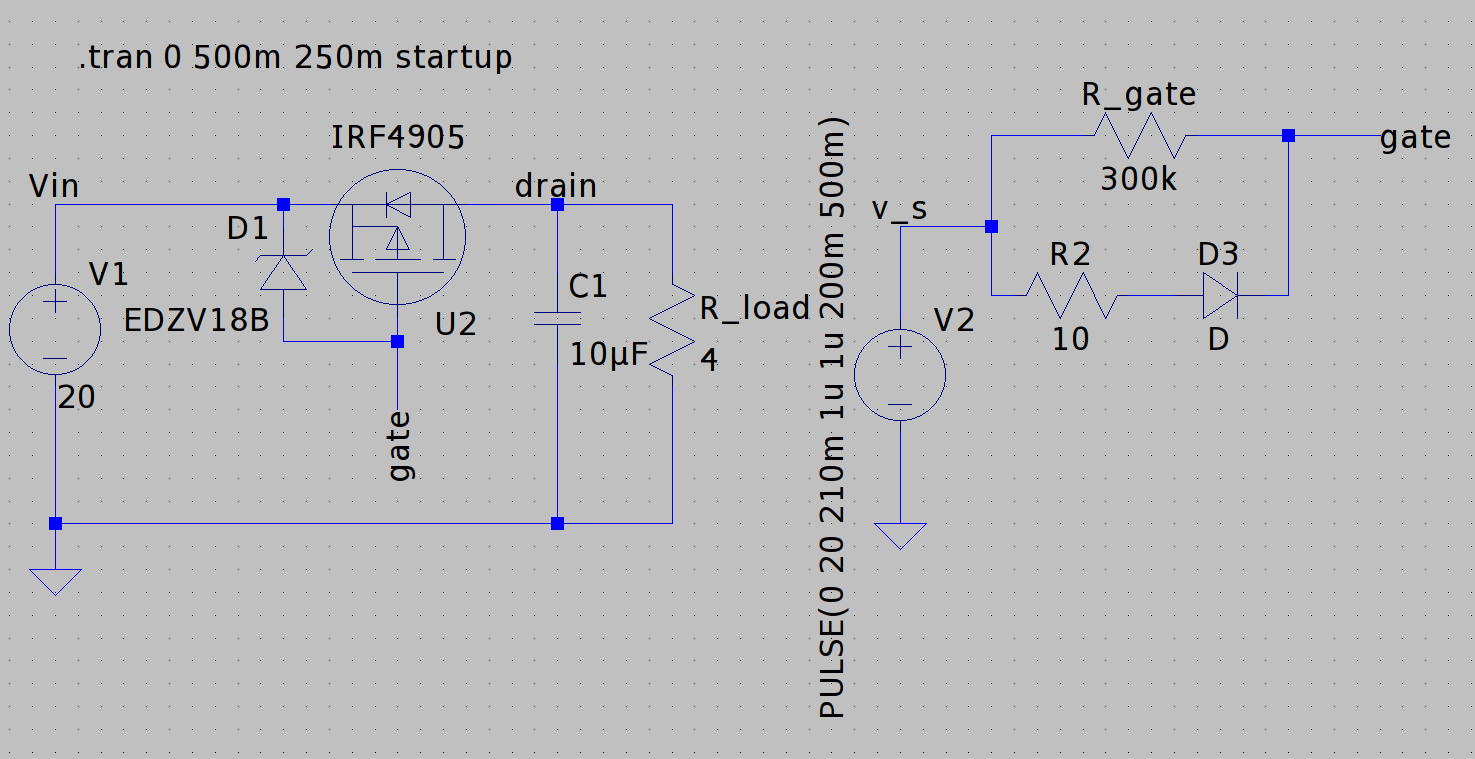
\includegraphics[width=\linewidth]{media/ideal_gate_drive.png}}
        \caption{Ideal gate driver circuit.}
        \label{fig:ideal_gate_drive}
    \end{figure}

    \begin{figure}[!h]
        \centerline{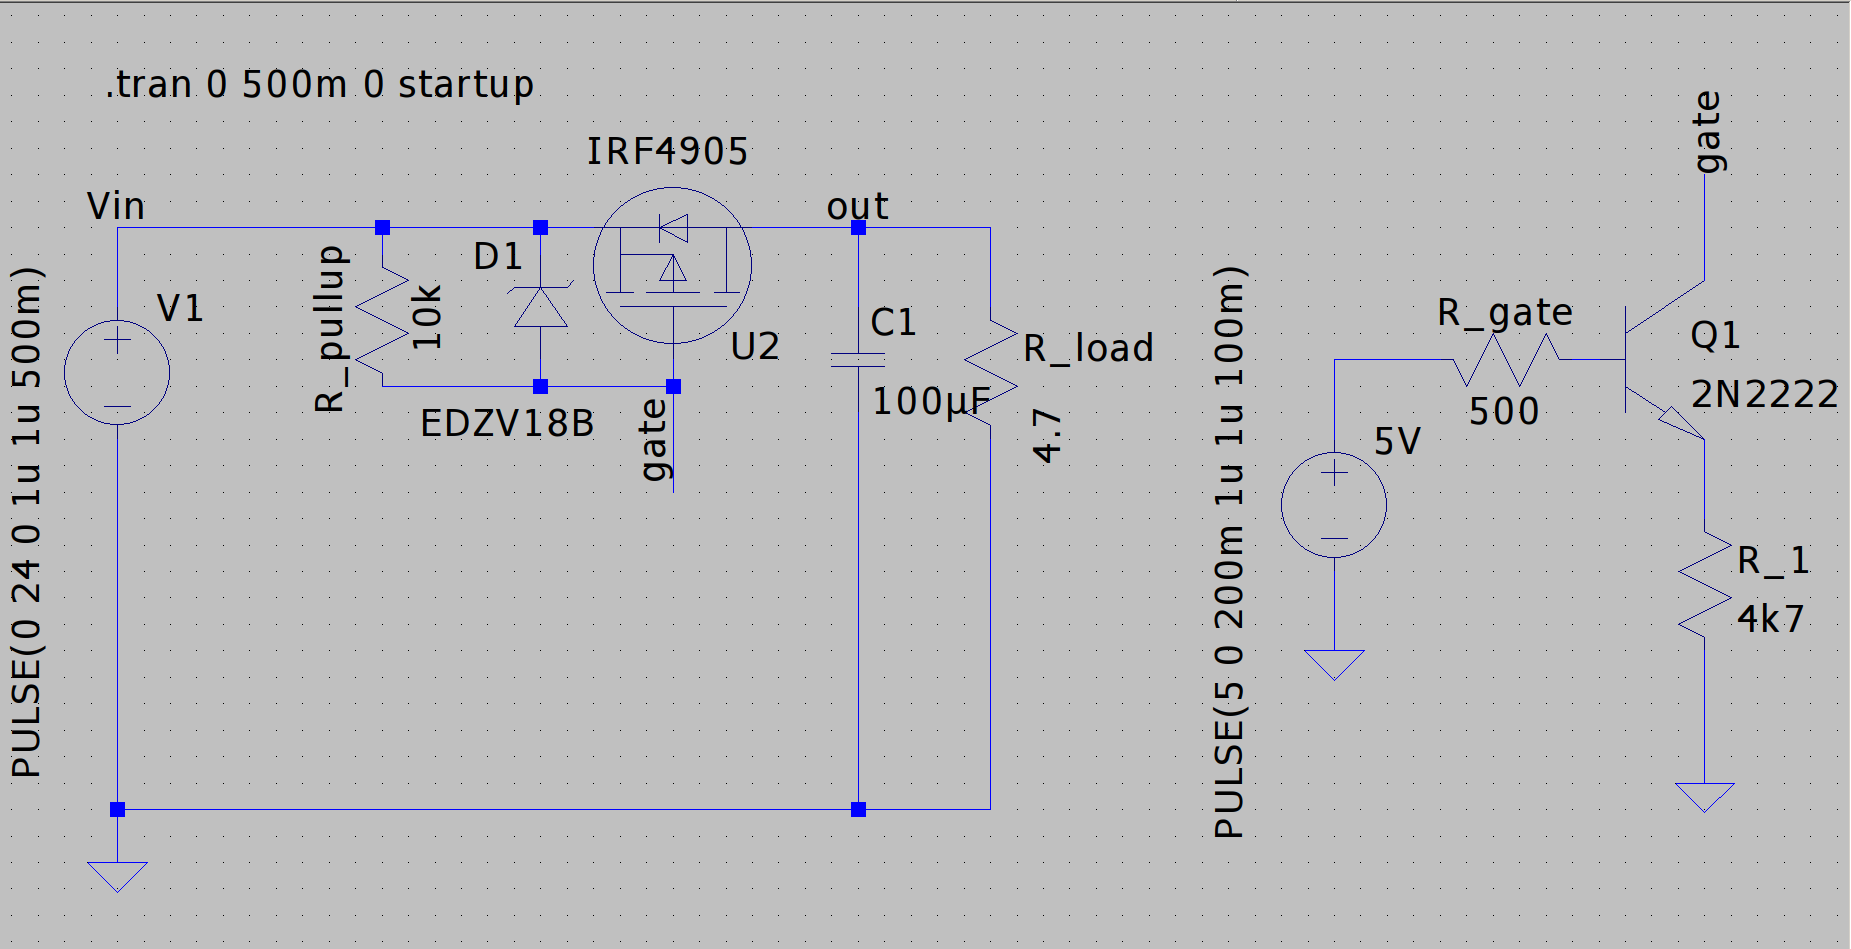
\includegraphics[width=\linewidth]{media/pmos_switch_npn.png}}
        \caption{Single-transistor gate driver circuit.} 
        \label{fig:single_transistor_gate_drive}
    \end{figure}

    \justify
    From the two example circuit, the following remarks can be made:
    \begin{enumerate}
        \item In the ideal example, the diode $D3$ allows for a larger current to be used for charging the gate which makes the turn-off event faster than turn-on (slow turn-on). This effect is desirable for application with capacitive load to reduce in-rush current.

        \item To replicate the slow turn-on effect in the single-transistor gate driver, the current through the $R_{pullup}$ while $Q_1$ is cut-off needs to be larger than that while $Q_1$ is in ohmic/saturation region, represented by equation \eqref{eq:slow_turn_on_condition}. This is generally plausible if the BJT is designed to be saturation region when turned on.
        
        \begin{equation} \label{eq:slow_turn_on_condition}
            I_{pullup}(\textbf{cut-off}) > I_{pullup}(\textbf{on})
        \end{equation}

        \item In MOSFET design, for a turn-on event, it is common to design to satisfy the following equation. It is so that the MOSFET is guaranteed to be in saturation region across the operating voltages.
        \begin{equation} \label{eq:deep_saturation_vgs}
            V_{gs} \approx -V_{in}
        \end{equation}

        Which leads to the following equation:

        \begin{equation} \label{eq:deep_saturation_condition}
            R_{E1} << R_{pullup} \Longleftrightarrow I_{pullup}(\textbf{cut-off}) > I_{pullup}(\textbf{on})
        \end{equation}
        
    \end{enumerate}

    \justify
    Equation \eqref{eq:slow_turn_on_condition} and \eqref{eq:deep_saturation_condition} are conflicting and cannot be achieved in the single-transistor gate driver. Thus, a push-pull topology or similar derivative can be used.

    \pagebreak
    \subsection{Push-pull topology} \label{sec:proposed_push_pull}

    \justify
    A push-pull topology uses a pair of transistors of different polarity that alternatively supply and absorb current from the load. In Figure \ref{fig:ideal_totem_pole}, a pair of NPN and PNP BJT is used. The use of opposite polarity transistor allows for a single digital signal $V_1$, swinging from $0V$ to $V_2$ can be used to turn on one transistor at a time.

    \begin{itemize}
        \item When $V_1=V_2$, $Q_2$ is on, while $Q_1$ is off. The load is connected to $V_2$.
        \item When $V_1=0V$, $Q_2$ is off, while $Q_1$ is on. The load is connected to ground.
    \end{itemize}

    \begin{figure}[!h]
        \centerline{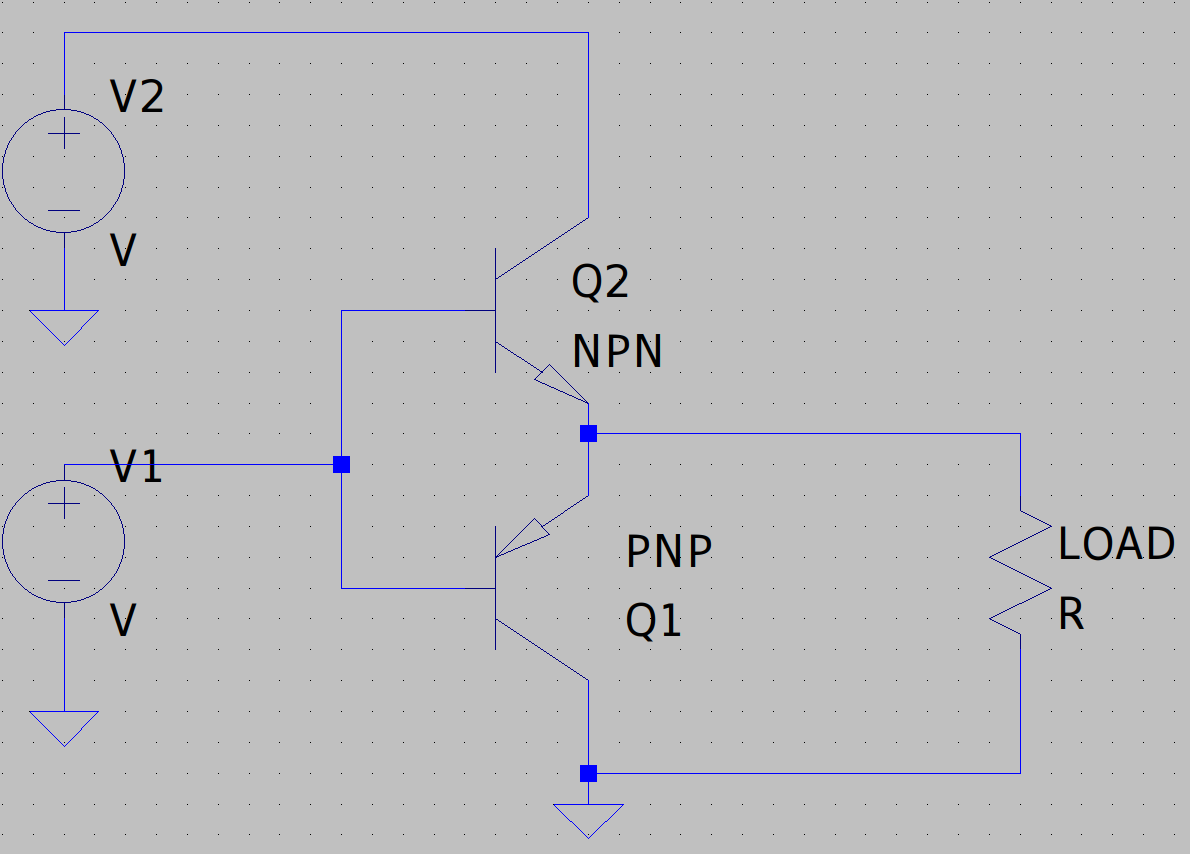
\includegraphics[scale=0.2]{media/ideal_totem_pole.png}}
        \caption{Ideal push-pull output.}
        \label{fig:ideal_totem_pole}
    \end{figure}

    \justify
    With this topology, a driver which satisfies the slow turn-on effect and Equation \eqref{eq:deep_saturation_vgs} can be achieved by providing different current path for charging/discharging the gate capacitance. In Figure \ref{fig:ideal_totem_pole_mod}, the desired effect is achieved by the diode $D_1$. However, the input voltage needs to swing from $0V$ to $V_2$ for the PNP transistor $Q_1$ to be cut-off properly.

    \begin{figure}[!h]
        \centerline{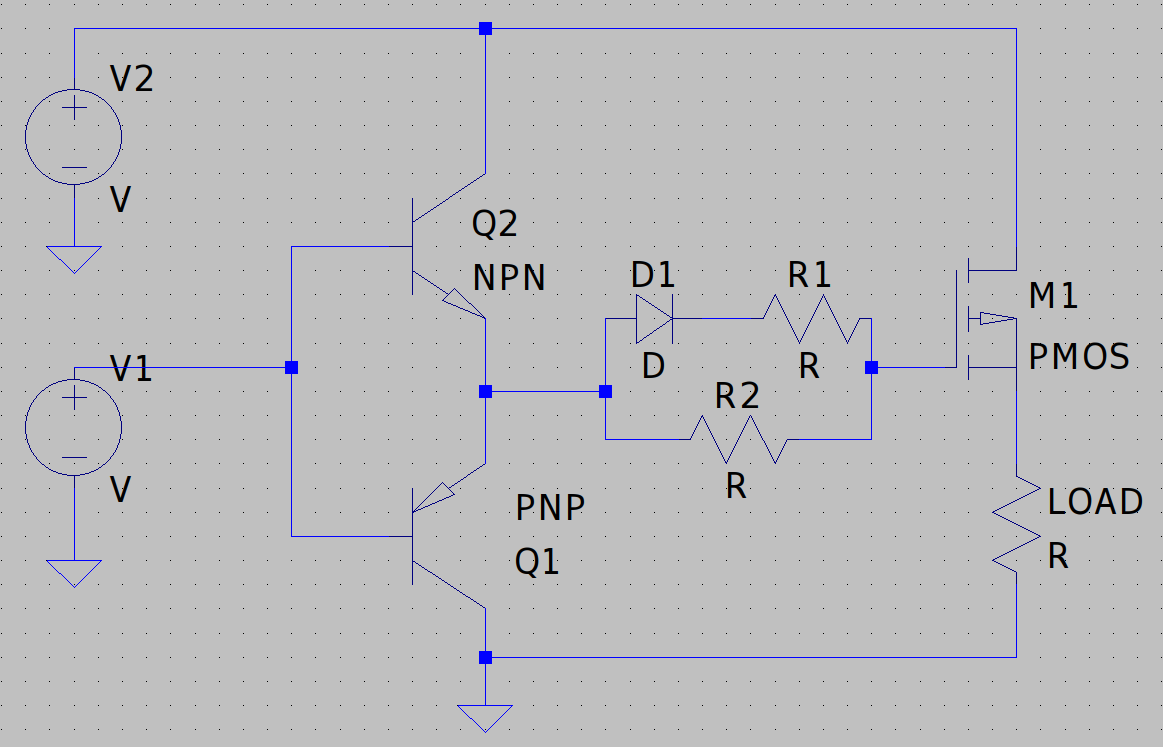
\includegraphics[scale=0.25]{media/ideal_totem_pole_mod.png}}
        \caption{Ideal push-pull MOSFET driver.}
        \label{fig:ideal_totem_pole_mod}
    \end{figure}

    \justify
    To mitigate the aforementioned downside, a design shown in Figure \ref{fig:proposed_gate_driver} using similar polarity BJTs (NPN) is proposed. There are two key differences in comparison to the former:
    \begin{itemize}
        \item  In an NPN, the base voltage only needs to be larger than $V_{BE}(saturated)\approx 0.7V$ for the transistor to be turned on. Thus, an input voltage range of $0V - 5V$ (suitable for MCU and logic ICs) is suitable for driving $Q_1$ to proper cut-off and saturation.
        \item $Q_2$ is not saturated. The gate is charged with $\beta I_{B2}$ which is controlled by resistor $R_2$.
    \end{itemize}

    \begin{figure}[!h]
        \centerline{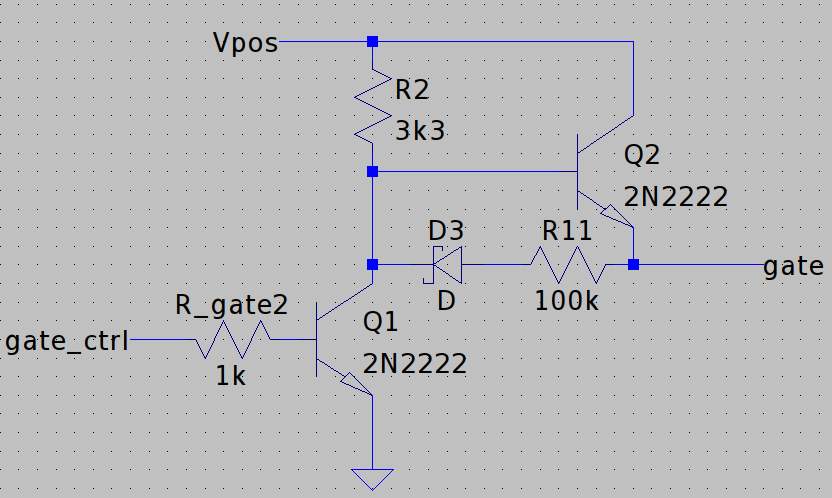
\includegraphics[width=\linewidth]{media/proposed_gate_driver.png}}
        \caption{Proposed push-pull MOSFET driver.}
        \label{fig:proposed_gate_driver}
    \end{figure}

    \justify
    Thus, the control of the MOSFET is as follows:
    \begin{enumerate}
        \item Input voltage is $0V$: $Q_1$ is cut-off, pulling up the base of $Q_2$ which turn it on and charge the gate capacitance.
        \item Input voltage is $5V$: $Q_1$ is turned on, pulling down the base of $Q_2$ which turn it off. The gate capacitance is discharged through $R_{11}$ and $Q_1$.
    \end{enumerate}
    
\end{document}